\documentclass[11pt]{article}

\usepackage[a4paper,margin=1in]{geometry}
\usepackage{amsmath,amssymb,amsthm}
\usepackage[colorlinks=true,linkcolor=blue,citecolor=blue,urlcolor=blue]{hyperref}
\usepackage{natbib}
\usepackage{booktabs}
\usepackage{graphicx}
\usepackage{xcolor}
\usepackage{tikz}

\newtheorem{theorem}{Theorem}[section]
\newtheorem{proposition}[theorem]{Proposition}
\newtheorem{corollary}[theorem]{Corollary}
\theoremstyle{definition}
\newtheorem{definition}[theorem]{Definition}
\newtheorem{observation}[theorem]{Observation}
\theoremstyle{remark}
\newtheorem{remark}[theorem]{Remark}
\newtheorem{caution}[theorem]{Caution}

\newcommand{\net}{c_{\mathrm{net}}}
\newcommand{\gross}{c_{\mathrm{gross}}}
\newcommand{\kcancel}{\kappa_{\mathrm{cancel}}}
\newcommand{\cond}{\mathrm{cond}}
\newcommand{\Fp}[1]{\mathbb{F}_{#1}}

\title{Two Blind Observables on a Signed Gauge Decomposition:\\
An Invariance-Audited Diagnostic Reading of the\\
Turok--Boyle Primordial Spectrum}
\author{Elias De Jes\'us\\ \small Independent Researcher\\ \small ORCID: \href{https://orcid.org/0009-0007-0190-9143}{0009-0007-0190-9143}\\ \small \texttt{dejesuselias10@gmail.com}}
\date{September 2026 --- Technical Note (third revision)}

\begin{document}
\maketitle

\begin{abstract}
Turok and Boyle compute the amplitude and spectral tilt of the primordial scalar perturbations
from the high-temperature trace-anomaly coefficient of the Standard Model,
$c_\beta = \tfrac{125}{108}\alpha_Y^2 - \tfrac{95}{72}\alpha_2^2 - \tfrac{49}{6}\alpha_3^2$
\citep{TurokBoyle2023}, a coefficient they in turn quote from \citet{ArnoldZhai1995}, evaluated at
Planck-scale couplings taken from \citet{Buttazzo2013}. This note records a diagnostic reading of
that object, and states plainly what is classical mathematics, what is imported physics, and what
is newly applied here. The physical question is: what do the two observables Turok and Boyle
extract actually reveal about the six-term signed sum that produces $c_\beta$, and what do they
necessarily conceal? The amplitude, proportional to $c_\beta^2$, reads only the magnitude of the
net signed sum across gauge channels and is blind both to that sum's internal decomposition and to
its sign. Under the heuristic assumptions Turok and Boyle use to connect spatial wavelength to
renormalization-group running, the tilt reads the dominant $SU(3)$ running combination $b_3\alpha_3$
alone. Neither observable resolves the channel decomposition. We quantify what is unresolved using
the classical signed-$L^1$ descriptors $\net = \sum_i c_i$ (total signed mass), $\gross = \sum_i
|c_i|$ (total variation mass), and the cancellation index $\kcancel = 1 - |\net|/\gross$. The
mathematics here is not new: reading $c$ as a discrete signed measure, $\net$ and $\gross$ are
exactly the Jordan-decomposition total signed and total variation masses \citep{Bogachev2007}, and
$\gross/|\net|$ is exactly the classical \emph{condition number of a sum} that governs
floating-point summation error \citep{Higham1993}, so $\kcancel = 1 - 1/\cond$ is a bounded,
invertible reparameterization of that textbook quantity, not a new invariant. What is applied here,
apparently for the first time to this coefficient, is a systematic identifiability audit built on
that classical vocabulary: we prove that only the net is fixed once the theory, truncation, and
scale are fixed, while $\gross$ and $\kcancel$ are functions of the sign-partition alone, satisfying
$\kcancel = 2\min(P,N)/(P+N)$ for the positive and negative masses $P,N$, monotonically
non-decreasing under any refinement crossing the sign boundary, and admitting no
decomposition-free value. Applied to Turok and Boyle's own coefficients, the gauge-factor
decomposition gives $\kcancel \approx 0.20$; refining each channel into its gauge-boson and matter
parts --- a split Turok and Boyle display for $SU(3)$ and which we show holds uniformly --- leaves
the net unchanged but raises $\kcancel$ to $0.64$; evaluating the same expression at the
electroweak scale gives $\kcancel \approx 0.002$. So $\kcancel \approx 0.20$ is a descriptor of one
stated decomposition at one stated scale and truncation, not a property of the Standard Model. We
also distinguish, throughout, between algebraic constructions used only to witness
non-identifiability (an arbitrary two-component split, a global sign flip) and the one
physically motivated refinement available here (gauge boson versus matter, at fixed order and
scale); the former are not alternative physically realizable decompositions of $c_\beta$. No claim
is made about the validity of the Turok--Boyle construction, which remains contested in the
refereed literature \citep{ClineHell2026}.
\end{abstract}

\tableofcontents

\section{Purpose, scope, and non-claims}
\label{sec:purpose}

Turok and Boyle propose that quantum zero-point fluctuations of dimension-zero fields seed the
primordial scalar perturbations, and compute both the amplitude and the spectral tilt in terms of
Standard Model couplings \citep{TurokBoyle2023}. Their amplitude is set by the high-temperature
trace-anomaly coefficient $c_\beta$ over an effective relativistic degree-of-freedom count; their
tilt is set by the running of the dominant gauge coupling at the Planck scale.

This note reads that result through a signed-decomposition and cancellation-index vocabulary
developed in a companion series on a different, purely mathematical partition construction
\citep{DeJesusThalesAtlas2026,DeJesusContextResolver2026,DeJesusPartitionFlows2026,DeJesusCompactness2026},
used strictly as coordinates. The aim is organizational: to say precisely which structures the
Turok--Boyle observables instantiate, and precisely where the analogy stops.

\paragraph{Non-claims.} This note does not validate, extend, derive, or critique the Turok--Boyle
construction. It does not claim that the signed-decomposition framework explains the primordial
spectrum. It asserts no physical mechanism beyond what the cited authors state, and proposes no new
cosmology. All physical inputs are theirs. It does not present $\kcancel$ as a new mathematical
invariant: Section~\ref{sec:descriptors} identifies it exactly with a classical quantity from
numerical linear algebra.

\paragraph{Relation to the first version.} An earlier version of this note \citep{DeJesusFirstVersion2026}
reported a cancellation index $\kcancel \approx 0.20$ for the gauge sector and described it as
characterizing that sector. That framing was too strong, and one sentence in it was simply wrong.
The present version retains the descriptors but subordinates them to an invariance audit
(Section~\ref{sec:audit}), works out an explicit alternative decomposition
(Section~\ref{sec:level2}), and corrects the sign description (Caution~\ref{caut:sign-correction}).
This third revision does not change any equation, theorem, or numerical value relative to the second;
it corrects the sourcing of the physical inputs, adds the condition-number identification of
$\kcancel$, labels every algebraic construction as a witness rather than a physical state, notes
the contested status of the Turok--Boyle mechanism in the refereed literature, and updates the
reproducibility appendix to the repository's current, consolidated implementation.

\section{The Turok--Boyle inputs, and their stated epistemic status}
\label{sec:inputs}

We quote only what is needed, and record how the authors themselves label each item and, where the
provenance chain runs further back than their own paper, where it actually originates.

\paragraph{(TB1) The coefficient.} The leading perturbative contribution to the high-temperature
trace $T_\beta \equiv \langle T^\lambda_\lambda\rangle_\beta$ of the Standard Model is, in Turok and
Boyle's Eq.~(4) \citep{TurokBoyle2023},
\begin{equation}
T_\beta^{\mathrm{SM}} = \left(\frac{125}{108}\alpha_Y^2 - \frac{95}{72}\alpha_2^2 -
\frac{49}{6}\alpha_3^2\right) T^4 \equiv c_\beta T^4, \qquad \alpha_i \equiv \frac{g_i^2}{4\pi}.
\label{eq:cbeta}
\end{equation}
Turok and Boyle state that this is their Eq.~(4), quoted from \citet{ArnoldZhai1995}, Eq.~(5.1) ---
the three-loop free energy of high-temperature QED and QCD with fermions. That is the coefficient's
true primary source, and \citet{ArnoldZhai1995} is cited directly here for the first time in this
note's history; the general SM group formula, applying \citeauthor{ArnoldZhai1995}'s per-factor
expression to each simple factor of the gauge group, is Turok and Boyle's own step. The full
Standard Model high-temperature pressure, including terms beyond gauge-plus-fermion, was computed
separately by \citet{GyntherVepsalainen2006}. Under Turok and Boyle's emergent-Higgs hypothesis no
scalar channels appear in \eqref{eq:cbeta}; Remark~\ref{rem:higgs-doublet} records exactly what that
omission costs relative to the textbook one-loop Standard Model beta functions.

\paragraph{(TB2) The couplings.} At the Planck scale, $\alpha_Y = 0.0181$, $\alpha_2 = 0.0203$,
$\alpha_3 = 0.0189$, giving $c_\beta = -0.0031$, with the $SU(3)$ contribution comprising $95\%$ of
the total \citep{TurokBoyle2023}. These couplings are not computed by Turok and Boyle themselves:
they are taken from \citet{Buttazzo2013}, via that paper's own Ref.~[37], and are cited to
\citet{Buttazzo2013} directly for the first time in this note's history.

\paragraph{(TB3) The amplitude.} With $N_0 = 36$ dimension-zero fields,
\begin{equation}
\mathcal{P}_\mathcal{R} = \frac{3\cdot 253}{7(2\pi)^4}\left(\frac{c_\beta}{N_{\mathrm{eff}}}\right)^2,
\qquad N_{\mathrm{eff}} = 106\tfrac{1}{4}.
\label{eq:amplitude}
\end{equation}
This is a derivation internal to Turok and Boyle's own framework, presented by them without
hedging.

\paragraph{(TB4) The tilt.} Focusing on the dominant $SU(3)$ contribution and leaving the flavour
number free, Turok and Boyle observe that the coefficient factorizes as
$T_\beta^{SU(3)} = -(12+5n_f)(11-\tfrac23 n_f)\alpha_3^2 T^4/36$, with the second factor
proportional to $\beta_{\alpha_3}/\alpha_3$ and the first accounted for by a thermal expectation
$\langle F^2\rangle_T$, and conclude
\begin{equation}
n_s - 1 = \frac{d\ln \mathcal{P}_\mathcal{R}}{d\ln k} = \frac{2\beta_{\alpha_3}}{\alpha_3} \approx
-\frac{7\alpha_3}{\pi} = -0.042.
\label{eq:tilt}
\end{equation}
The authors explicitly label this a \emph{heuristic analysis} and caution that it rests on key
theoretical assumptions they have yet to verify: specifically, that the running factor depends on
the spatial wavelength at which the dimension-zero field couples to the plasma, and a further final
assumption about extrapolation from the Planck scale. Section~\ref{sec:tiers} takes this at face
value.

\paragraph{Contested status.} The Turok--Boyle proposal is a February 2023 arXiv preprint with, as
of this revision, no located journal version. Its central ingredient --- dimension-zero scalar
fields --- has since been examined in the refereed literature by \citet{ClineHell2026}, who
identify pathologies in the mechanism this note's subject coefficient is meant to support. This
note takes no position on that critique; the diagnostic below concerns what the two stated
observables can resolve about a given decomposition, independently of whether the underlying
mechanism survives scrutiny. A reader should know the proposal is contested, not merely unverified
by its own authors.

\section{The two-level structure of the coefficient}
\label{sec:twolevel}

Turok and Boyle display the plasma/$\beta$ factorization only for the $SU(3)$ channel. It holds
for all three, and stating it in that generality is what makes the rest of this note coherent.

\begin{proposition}[Uniform positive-factor/$\beta$-coefficient decomposition]
\label{prop:factorization}
Write $b_a := \tfrac{11}{3}C_A^{(a)} - \tfrac43 S_F^{(a)}$ for the combination of group invariants
using the data Turok and Boyle quote explicitly \citep{TurokBoyle2023} ($C_A = 0,2,3$ and $S_F =
5,3,3$ for $U(1)_Y$, $SU(2)_L$, $SU(3)_c$). Then each term of \eqref{eq:cbeta} factorizes exactly
as
\begin{equation}
c_a = -P_a \alpha_a^2 b_a, \qquad P_{U(1)} = \frac{25}{144}, \quad P_{SU(2)} = \frac{19}{48}, \quad
P_{SU(3)} = \frac76,
\label{eq:factorization}
\end{equation}
with $b_{U(1)} = -\tfrac{20}{3}$, $b_{SU(2)} = \tfrac{10}{3}$, $b_{SU(3)} = 7$. All three factors
$P_a$ are strictly positive.
\end{proposition}

\begin{proof}
Direct substitution. For $SU(3)$: $b = \tfrac{11}{3}\cdot 3 - \tfrac43\cdot 3 = 11-4 = 7$, and
$-\tfrac76\cdot 7 = -\tfrac{49}{6}$, reproducing the third coefficient of \eqref{eq:cbeta} and
agreeing with $-(12+5n_f)(11-\tfrac23 n_f)/36 = -49/6$ at $n_f=6$. For $SU(2)$:
$b = \tfrac{22}{3}-4 = \tfrac{10}{3}$, and $-\tfrac{19}{48}\cdot\tfrac{10}{3} = -\tfrac{95}{72}$.
For $U(1)_Y$: $C_A=0$ gives $b = -\tfrac{20}{3}$, and $-\tfrac{25}{144}\cdot(-\tfrac{20}{3}) =
+\tfrac{125}{108}$.
\end{proof}

\begin{remark}[$b_a$ is the Arnold--Zhai gauge-plus-fermion combination, not the textbook one-loop
Standard Model beta function]
\label{rem:higgs-doublet}
Each $b_a$ above reproduces Turok and Boyle's own $(C_A, S_F)$ data exactly, and the values are not
in question. They are \emph{not}, however, the textbook Standard Model one-loop gauge beta
coefficients, which in Standard-Model hypercharge normalization are $b_{U(1)} = -\tfrac{41}{6}$ and
$b_{SU(2)} = \tfrac{19}{6}$. Each differs from the value used here by exactly $\tfrac16$ --- the
contribution of a fundamental Higgs doublet, absent from the Arnold--Zhai gauge-plus-fermion
high-temperature expression \citep{ArnoldZhai1995} because it is a QED/QCD-type computation with no
scalar sector. This omission is not an inconsistency: it is exactly what Turok and Boyle's own
premise requires, since their construction needs the Higgs doublet to be \emph{emergent} rather
than fundamental. No equation or numerical value in this note is affected; the point is only that a
reader who checks $b_a$ against a textbook one-loop Standard Model beta function will find a
mismatch, and should understand why.
\end{remark}

\begin{caution}[Algebraic factorization versus physical interpretation]
\label{caut:algebraic}
For $SU(3)$, Turok and Boyle interpret the positive factor physically, through the thermal
expectation $\langle F^2\rangle_T$ of the gluon field strength, and it is that interpretation which
motivates calling it a plasma factor. For $U(1)_Y$ and $SU(2)_L$, Proposition~\ref{prop:factorization}
establishes only the analogous algebraic factorization: $P_a$ is defined as the ratio $-c_a/(\alpha_a^2
b_a)$, and its positivity is a computed fact, not a sourced physical identification. No claim is
made here that $P_{U(1)}$ and $P_{SU(2)}$ are thermal expectation values, unless such an
identification is supplied by the underlying thermal-field-theory calculation. We were unable to
write the three values $25/144$, $19/48$, $7/6$ as a simple closed form in the group invariants
$(d_A, C_A, S_F)$; this is not a proof that none exists, but it is a reason not to present the
algebraic rearrangement as a uniform physical structure. Nothing below depends on the
interpretation --- only on $P_a > 0$.
\end{caution}

\begin{corollary}[Where the signs come from]
\label{cor:signs}
Since $P_a > 0$ and $\alpha_a^2 > 0$, the sign of every channel is carried entirely by $-b_a$. The
hypercharge channel is positive precisely because $C_A^{(U(1))} = 0$: an abelian factor has no
gauge self-coupling, so its $\beta$-coefficient receives only the matter (screening) contribution.
The two non-abelian channels are negative because antiscreening dominates. The mixed sign pattern
of \eqref{eq:cbeta} is therefore not a numerical accident of the Planck-scale couplings; it is the
abelian/non-abelian distinction.
\end{corollary}

Proposition~\ref{prop:factorization} exhibits $c_\beta$ as a two-level object. Level~1 is the
partition into three gauge factors. Level~2 resolves each factor into a positive prefactor times a
$\beta$-coefficient which is itself a difference, $\tfrac{11}{3}C_A - \tfrac43 S_F$, of an
antiscreening and a screening piece. Both levels are mathematically legitimate; Section~\ref{sec:level2}
shows they give different answers for $\kcancel$, and Section~\ref{sec:audit} explains why that had
to happen.

\section{Reading 1: what each observable actually reads}
\label{sec:reading1}

\begin{observation}[Two different blindnesses]
\label{obs:blindness}
Relative to the structure of Proposition~\ref{prop:factorization}:
\begin{enumerate}
\item[(i)] The amplitude \eqref{eq:amplitude} is an even function of the net,
$\mathcal{P}_\mathcal{R} \propto c_{\mathrm{net}}^2$, so it depends on $|c_\beta|$ and on nothing
else about the decomposition. It reads all three channels, but only through the magnitude of their
signed total; it is blind both to how that total is composed and to whether it is positive or
negative. The latter blindness is not an artefact of bookkeeping: in \citep{TurokBoyle2023} the
sign of $c_\beta$ flips the sign of the coupling $c_\chi$ and hence of $\mathcal R$, but $\delta\chi$
is a zero-mean Gaussian field, so the sign is invisible in the two-point function that defines
$\mathcal{P}_\mathcal{R}$.
\item[(ii)] The tilt \eqref{eq:tilt} is $2\beta_{\alpha_3}/\alpha_3 = -b_{SU(3)}\alpha_3/\pi$, so it
reads the combination $b_{SU(3)}\alpha_3$, not the $\beta$-coefficient alone. It is independent of
the positive prefactor $P_{SU(3)}$ and of the $U(1)_Y$ and $SU(2)_L$ channels entirely. This holds
only under the heuristic wavelength-to-running assumptions of \citep{TurokBoyle2023}.
\end{enumerate}
Neither observable resolves the channel decomposition, and the two fail to resolve it in different
directions: the amplitude aggregates across channels, retains both factors, and discards the sign;
the tilt isolates one channel and discards its positive prefactor.
\end{observation}

\begin{caution}[The complementarity claim, corrected]
\label{caut:complementarity}
The first version of this note described the amplitude and tilt as occupying complementary slots
of one object, in the same diagnostic form as coupling/asymmetry pairs used elsewhere in the
author's own partition-construction series. That overstated the parallel in two ways, and the
overstatement is now withdrawn. First, the pair is nested, not complementary: the tilt reads a
strict sub-factor of what the amplitude reads, since $b_{SU(3)}$ appears in both, while the
amplitude additionally carries $P_a$ and the subdominant channels. Second, magnitude/logarithmic-derivative
pairs are generic --- every observable and its running form one --- so recognizing that pattern here
has limited discriminating power and should be read as shared vocabulary, not as evidence of shared
structure.
\end{caution}

\section{The signed context and its descriptors}
\label{sec:descriptors}

\begin{definition}[Signed $L^1$ descriptors]
\label{def:descriptors}
For a finite family of signed contributions $\{c_i\}$ set
\begin{equation}
\net = \sum_i c_i, \qquad \gross = \sum_i |c_i|, \qquad \kcancel = 1 - \frac{|\net|}{\gross} \in
[0,1],
\label{eq:descriptors}
\end{equation}
with $\kcancel$ undefined when $\gross = 0$. Note $\kcancel = 1$ exactly when $\net = 0$, i.e.\
under total cancellation; the physical case treated here has $\net \ne 0$ and hence $\kcancel < 1$.
Writing $P = \sum_{c_i>0} c_i$ and $N = -\sum_{c_i<0} c_i$ for the positive and negative masses,
\begin{equation}
\kcancel = \frac{2\min(P,N)}{P+N}.
\label{eq:kappa-pn}
\end{equation}
\end{definition}

\begin{proof}[Proof of \eqref{eq:kappa-pn}]
$\net = P-N$ and $\gross = P+N$, so $1 - |P-N|/(P+N) = \big(P+N-|P-N|\big)/(P+N) = 2\min(P,N)/(P+N)$.
\end{proof}

Identity \eqref{eq:kappa-pn} is the structural fact on which the whole of Section~\ref{sec:audit}
turns: $\kcancel$ is a function of the two sign-class totals and of nothing else. It does not know
how many channels there are, or which is which.

\begin{proposition}[$\kcancel$ is a bounded reparameterization of the classical condition number of
a sum]
\label{prop:condition-number}
Define $\cond := \gross/|\net|$, for $\net \ne 0$. Then
\begin{equation}
\kcancel = 1 - \frac1\cond, \qquad \cond = \frac{1}{1-\kcancel},
\label{eq:condition-number}
\end{equation}
and both directions are exact. The quantity $\cond$ is precisely the factor in the standard
error bound for floating-point summation, $\big|\widehat{\sum x_i} - \sum x_i\big| \lesssim
(n-1)u\sum|x_i|$, restated relative to $|\sum x_i|$ \citep{Higham1993}; it is universally called
the condition number of the summation problem $\{c_i\} \mapsto \sum_i c_i$.
\end{proposition}

\begin{proof}
Immediate from Definition~\ref{def:descriptors}: $1 - 1/\cond = 1 - |\net|/\gross = \kcancel$, and
solving for $\cond$ gives the second form.
\end{proof}

\begin{remark}
\label{rem:condition-number-interpretation}
Proposition~\ref{prop:condition-number} is the reason $\kcancel$ is not presented here as a new
invariant. For $\net\neq0$, $\cond$ is always a finite real number in $[1,\infty)$ --- the triangle
inequality gives $\gross\ge|\net|>0$, so $\cond\ge1$, with equality iff the family is
sign-homogeneous --- and $\kcancel=1-1/\cond$ is an exact, invertible, monotone rescaling of that
half-open interval onto $\kcancel\in[0,1)$; the value $\cond=\infty$ is never attained by any actual
finite family with $\net\neq0$, only approached in the limit of Theorem~\ref{thm:monotonicity}(vi).
The boundary case $\net=0$, $\gross>0$ is separate, not a limit of this formula: there
$\cond=\gross/|\net|$ is undefined (division by zero), while $\kcancel=1$ exactly, directly from
Definition~\ref{def:descriptors} rather than from Proposition~\ref{prop:condition-number}. The two
descriptions agree in spirit --- $\cond\to\infty$ corresponds to $\kcancel\to1$ --- but only the
$\net\neq0$ case is literally a rescaling of a well-defined $\cond$. The only thing gained by
working with $\kcancel$ rather than $\cond$ directly, on their common domain, is boundedness. Every
mathematical result below --- Theorem~\ref{thm:monotonicity} in particular --- can be read
equivalently as a statement about how the summation condition number of $\{c_i\}$ changes under
refinement, coarsening, and relabelling of a fixed sum, which is the natural language in which
numerical analysts already discuss such sums \citep{Higham1993}.
\end{remark}

\begin{proposition}[Marginal blindness, algebraic form]
\label{prop:marginal-blindness}
Let $O = f(\net)$ for some $f$. Then:
\begin{enumerate}
\item[(i)] $O$ cannot distinguish two signed families with equal net, whatever their gross
magnitudes or cancellation indices. In particular the amplitude assigns the same value to
decomposition \eqref{eq:cbeta}, with $\kcancel = 0.20$, as to a single channel of the same net with
$\kcancel = 0$.
\item[(ii)] If in addition $f$ is even --- as it is for the amplitude, $\mathcal{P}_\mathcal{R}
\propto c_{\mathrm{net}}^2$ --- then $O$ satisfies $O(\net) = O(-\net)$ and is a function of
$|\net|$ alone, so it is blind to the overall sign as well as to the decomposition.
\end{enumerate}
\end{proposition}

\begin{proof}
(i) is immediate, since $f$ is a function of $\net$ alone. (ii) is the definition of an even
function.
\end{proof}

\begin{remark}[This proposition is nearly trivial, and should be labelled as such]
\label{rem:trivial}
Proposition~\ref{prop:marginal-blindness} is an observation about functions of a sum: it is the
elementary statement that a many-to-one observation map cannot be inverted, a standard
non-identifiability fact \citep{Rothenberg1971}. It carries no information beyond the definition of
$\mathcal{P}_\mathcal{R}$. Its interest lies entirely in what it licenses one to ask --- how much
structure is hidden, and relative to what --- and that question is answered by
Sections~\ref{sec:audit} and~\ref{sec:level2}, not by the proposition. It should not be cited as a
result.
\end{remark}

\begin{remark}[The two blindnesses are logically independent]
\label{rem:logical-independence}
Sign blindness is not implied by decomposition blindness: an observable $O = \net$ resolves the
sign while remaining blind to the decomposition. Conversely, an observable of $\gross$ alone would
be sign-blind while sensitive to the decomposition. The amplitude happens to suffer both. Note also
that $\kcancel$ itself is invariant under the global flip $c_i \mapsto -c_i$, which interchanges $P$
and $N$ and leaves \eqref{eq:kappa-pn} unchanged; so the descriptors of Definition~\ref{def:descriptors}
restore the information the amplitude loses about the decomposition, but not the information it
loses about the sign. The global sign flip used to establish this is an \emph{algebraic witness}: it
is not a physically available operation on the Standard Model coefficient $c_\beta$, whose sign is
fixed once the theory and scale are fixed.
\end{remark}

\begin{remark}[Logical independence of amplitude and tilt is stronger than stated, but is not
physical independence]
\label{rem:functional-independence}
The amplitude and tilt are also functionally independent on the three-coupling space, not merely
independent as abstract functionals of different arguments. Treating $(\alpha_Y,\alpha_2,\alpha_3)$
as free: holding $c_\beta = -0.003082$ fixed and moving $\alpha_3$ from $0.0189$ to $0.0210$, with
$\alpha_Y$ solved to compensate (giving $\alpha_Y \approx 0.0303$), moves $n_s-1$ from $-0.042112$
to $-0.046792$; holding $\alpha_3$ fixed and moving $\alpha_2$ over $0.018$--$0.023$ moves $c_\beta$
over $-0.002966$ to $-0.003236$ with the tilt exactly unchanged, since \eqref{eq:tilt} does not
depend on $\alpha_2$ at all. So the two observables are genuinely functionally independent on the
three-coupling space, not merely independent as abstract functionals. This is, however, a statement
about the \emph{observation map of the model family}: at the Standard Model Planck point the three
couplings are determined, not free, so the witnesses above describe what the map $(\alpha_Y,\alpha_2,
\alpha_3) \mapsto (c_\beta, n_s-1)$ can and cannot separate, not a degeneracy among physically
realized states. (The family is constrained: at $\alpha_3 = 0.017$ there is no real $\alpha_Y$
holding $c_\beta$ fixed.)
\end{remark}

\begin{remark}[Signed $L^1$ is not a Fisher simplex]
\label{rem:not-fisher}
A companion construction on a different, purely mathematical partition \citep{DeJesusContextResolver2026}
proves a context-resolver theorem for non-negative context pieces $c_i \ge 0$ with $\sum_i c_i = c$,
where a warped-product factor telescopes and subcomponent structure lives in Fisher information
geometry on the resulting probability simplex. The positivity hypothesis is essential and fails
here: by Corollary~\ref{cor:signs} the gauge decomposition is genuinely signed. Consequently the
present statement is the signed analogue of marginal blindness, not an instance of it: it is
algebraic (Proposition~\ref{prop:marginal-blindness}) rather than a telescoping identity, it comes
with no Fisher-geometric content, and the descriptors of Definition~\ref{def:descriptors} --- the
Jordan-decomposition total variation mass, not a Fisher metric --- replace the simplex invariants.
A Fisher treatment would require either normalizing the absolute contributions, which discards
exactly the sign information at issue, or a genuine signed-context extension of the resolver
theorem; that extension is not attempted here.
\end{remark}

\section{Invariance audit}
\label{sec:audit}

This section asks, for each descriptor of Definition~\ref{def:descriptors}, what must be held
fixed before the quantity is well defined.

\begin{definition}[Refinement and coarsening]
\label{def:refinement}
A family $\{c_j'\}$ refines $\{c_i\}$ if there is a surjection $\pi$ from the index set of $c'$ onto
that of $c$ with $c_i = \sum_{\pi(j)=i} c_j'$ for every $i$; $\{c_i\}$ then coarsens $\{c_j'\}$. A
refinement is \emph{sign-homogeneous} if every group $\{c_j' : \pi(j)=i\}$ consists of terms of one
sign.\footnote{Precisely: a group is sign-homogeneous when no two of its nonzero terms have
strictly opposite signs; adjoining zero terms changes nothing.}
\end{definition}

\begin{theorem}[Monotonicity, and non-existence of a canonical value]
\label{thm:monotonicity}
Let $\{c_j'\}$ refine $\{c_i\}$. Then
\begin{enumerate}
\item[(i)] $\net$ is unchanged;
\item[(ii)] $\gross' \ge \gross$, with equality if and only if the refinement is sign-homogeneous;
\item[(iii)] consequently $\kcancel' \ge \kcancel$, with equality under the same condition;
\item[(iv)] $\kcancel$ is a symmetric function of the multiset $\{c_i\}$ and hence invariant under
relabelling;
\item[(v)] merging channels of opposite sign strictly decreases $\kcancel$;
\item[(vi)] for any family with $\net \ne 0$ and any $\varepsilon>0$ there is a refinement with
$\kcancel > 1-\varepsilon$, and coarsening to a single channel gives $\kcancel = 0$. Hence over all
decompositions of a fixed net, $\kcancel$ ranges over the whole of $[0,1)$ and possesses no
decomposition-free extremum.
\end{enumerate}
\end{theorem}

\begin{proof}
(i) is the definition of refinement. (ii) By the triangle inequality $|c_i| = |\sum_{\pi(j)=i}
c_j'| \le \sum_{\pi(j)=i}|c_j'|$, with equality iff the terms in the group share a sign; summing
over $i$ gives the claim. (iii) $\kcancel = 1-|\net|/\gross$ is strictly increasing in $\gross$ at
fixed $\net \ne 0$, so (ii) transfers. (iv) is immediate from \eqref{eq:kappa-pn}. (v) is (iii) read
in reverse. For (vi), choose any component $c_r$ and refine it as $c_r = (c_r+X) + (-X)$ for
$X > \max\{0,-c_r\}$, which is a refinement in the sense of Definition~\ref{def:refinement} because
the two pieces are assigned to $c_r$ and sum to it. The net is unchanged, while the gross increases
by $|c_r+X|+X-|c_r| = c_r+2X-|c_r| \to \infty$ as $X\to\infty$, so $\kcancel' \to 1$. Coarsening the
whole family to $\{\net\}$ gives $\gross = |\net|$ and $\kcancel = 0$. More generally, for fixed
$\net = n \ne 0$ the two-component decompositions $\big(\tfrac{G+n}{2}, -\tfrac{G-n}{2}\big)$,
$G \ge |n|$, have net $n$ and gross $G$, realizing every value $\kcancel = 1-|n|/G$ in $[0,1)$.
\end{proof}

\begin{remark}[Every construction in Theorem~\ref{thm:monotonicity}(vi) is an algebraic witness,
not a physical decomposition]
\label{rem:witness}
The refinement $c_r = (c_r+X)+(-X)$ and the two-component family $\big(\tfrac{G+n}{2},
-\tfrac{G-n}{2}\big)$ are constructed purely to demonstrate that $\kcancel$ has no
decomposition-free supremum; they are not claimed to correspond to any physically realizable
splitting of a Standard Model gauge-sector coefficient. The distinction matters because it is easy
to conflate ``$\kcancel$ can be made arbitrarily close to $1$ by \emph{some} refinement'' with
``the gauge sector's cancellation is arbitrarily close to total'' --- the theorem licenses only the
first statement. The one refinement in this note that \emph{is} physically motivated ---
gauge-boson versus matter, at fixed perturbative order and scale --- is treated separately, in
Section~\ref{sec:level2}, precisely because it is not one of these algebraic witnesses.
\end{remark}

\begin{remark}[The threshold in (vi) is not cosmetic]
\label{rem:threshold}
The condition $X > \max\{0,-c_r\}$ is exactly what forces the refinement to cross the sign
boundary. Refining the strong channel of \eqref{eq:cbeta}, for which $c_r<0$, with
$X=10^{-3} < -c_r$ leaves both pieces negative: the refinement is sign-homogeneous, the gross is
unchanged, and $\kcancel$ stays at $0.1975$, in accordance with (ii). Taking $X=10^{-2}$ crosses the
threshold and gives $\kcancel = 0.829$; $X=1$ gives $\kcancel = 0.998$.
\end{remark}

Theorem~\ref{thm:monotonicity} is the reason the first version of this note overstated its case: it
shows that $\kcancel$ is not a property of a physical system but of a stated resolution of that
system, and that no refinement is distinguished by the formalism itself. Two further dependences,
which are not decomposition choices at all, must also be fixed.

\paragraph{Truncation.} Coefficients \eqref{eq:cbeta} are the leading $O(\alpha^2)$ perturbative
contribution; the Standard Model free energy is known to higher order. At higher orders the
expansion contains mixed-coupling terms ($\alpha_Y\alpha_2$, $\alpha_2\alpha_3$, and, absent the
emergent-Higgs hypothesis, terms in the top Yukawa and the Higgs quartic), which belong to no
single gauge factor. Beyond one loop the gauge beta functions of a general quantum field theory mix
different gauge couplings, Yukawa couplings, and scalar couplings \citep{MachacekVaughn1983}; the
Standard Model's own three-loop gauge beta functions have been computed explicitly and confirm this
structure \citep{Mihaila2012}. The one-channel-per-simple-factor decomposition therefore ceases to
be closed and canonical beyond leading order: accommodating such terms requires either interaction
channels indexed by pairs of factors, or a stated convention assigning each mixed term to one
factor. This is not an impossibility --- decompositions still exist --- but it means the channel set
is itself a further modelling choice, and by Theorem~\ref{thm:monotonicity} that choice moves
$\kcancel$.

\paragraph{Renormalization scale.} Each $c_a$ depends on $\mu$ through $\alpha_a(\mu)$, and the
three couplings run at different rates, so $\kcancel$ runs too. Table~\ref{tab:scale} records the
effect.

\begin{table}[t]
\centering
\small
\begin{tabular}{@{}l r r r r r@{}}
\toprule
Scale & $\alpha_Y$ & $\alpha_2$ & $\alpha_3$ & $\net$ & $\kcancel$ (level 1) \\
\midrule
Planck & 0.0181 & 0.0203 & 0.0189 & $-3.08\times 10^{-3}$ & 0.197 \\
Electroweak & 0.0102 & 0.0338 & 0.1184 & $-1.16\times 10^{-1}$ & 0.002 \\
\bottomrule
\end{tabular}
\caption{Scale dependence of the level-1 index, evaluating \eqref{eq:cbeta} with couplings at two
scales. The electroweak row is illustrative of the running only: it applies the same
high-temperature expression at a much lower scale, where the perturbative hierarchy and the
applicability of the high-$T$ expansion both differ, and the electroweak couplings used here are
textbook values not drawn from a cited source (unlike the Planck row, which is
\citet{Buttazzo2013} via \citet{TurokBoyle2023}). The point is the two orders of magnitude, not the
second digit.}
\label{tab:scale}
\end{table}

\paragraph{Scheme and normalization.} At one loop the $b_a$ are scheme-independent, and the choice
between Standard-Model and grand-unified normalization of hypercharge leaves $c_a$ invariant, since
$g_1 \mapsto \lambda g_1$ is compensated by $b_1 \mapsto b_1/\lambda^2$. Beyond one loop, scheme
dependence enters through both the $\beta$ coefficients and the extracted couplings. Basis changes
are not a source of ambiguity here: the gauge group is a direct product of simple factors and each
contributes a distinct gauge-invariant operator, so there is no mixing to choose. (This last
stability would fail for extensions with several abelian factors, where kinetic mixing makes the
abelian split basis-dependent.)

\begin{table}[t]
\centering
\small
\begin{tabular}{@{}p{0.34\linewidth} p{0.20\linewidth} p{0.36\linewidth}@{}}
\toprule
Operation & Effect on $\kcancel$ & Reason \\
\midrule
Relabelling channels & unchanged & Theorem~\ref{thm:monotonicity}(iv) \\
Merging channels of like sign & unchanged & Theorem~\ref{thm:monotonicity}(ii) \\
Merging channels of opposite sign & decreases & Theorem~\ref{thm:monotonicity}(v) \\
Splitting into like-sign pieces & unchanged & Theorem~\ref{thm:monotonicity}(ii) \\
Splitting across the sign boundary & increases, unbounded & Theorem~\ref{thm:monotonicity}(iii),(vi) \\
Global sign flip $c_i \mapsto -c_i$ & unchanged & interchanges $P,N$ in \eqref{eq:kappa-pn} \\
Change of basis & unchanged & direct-product gauge group; no mixing at this order \\
Hypercharge normalization (SM $\leftrightarrow$ GUT) & unchanged & $g_1\mapsto\lambda g_1$, $b_1 \mapsto b_1/\lambda^2$ \\
Renormalization scheme & unchanged at one loop & one-loop $b_a$ scheme-independent \\
Loop order / truncation & changes, channel set not closed & \citet{MachacekVaughn1983,Mihaila2012} \\
Renormalization scale $\mu$ & changes, strongly & Table~\ref{tab:scale} \\
\bottomrule
\end{tabular}
\caption{Invariance audit for the cancellation index. The same classification applies to $\gross$;
$\net$ is unchanged by every operation in the first six rows and changes only with truncation and
scale.}
\label{tab:audit}
\end{table}

\section{An alternative, physically meaningful decomposition}
\label{sec:level2}

Theorem~\ref{thm:monotonicity} says refinement can change $\kcancel$. The relevant question is
whether any \emph{natural} refinement does. It does, and the refinement in question is displayed in
the Turok--Boyle paper itself.

By Proposition~\ref{prop:factorization}, $c_a = -P_a\alpha_a^2\big(\tfrac{11}{3}C_A^{(a)} -
\tfrac43 S_F^{(a)}\big)$. The bracket is a difference of an antiscreening (gauge-boson loop) term
and a screening (matter loop) term of opposite signs --- exactly the split Turok and Boyle write out
as $(11-\tfrac23 n_f)$ for $SU(3)$. Resolving it gives the level-2 family
\begin{equation}
c_a^{\mathrm{gauge}} = -P_a\alpha_a^2 \cdot \tfrac{11}{3}C_A^{(a)}, \qquad
c_a^{\mathrm{matter}} = +P_a\alpha_a^2 \cdot \tfrac43 S_F^{(a)}.
\label{eq:level2}
\end{equation}
This is a legitimate refinement at one loop, where $b_a$ literally is that sum; it is diagrammatic
bookkeeping, not a claim that the two pieces are separately observable.

\begin{caution}[Correction of a factual error in the previous version]
\label{caut:sign-correction}
The first version of this note stated, in its abstract, in its main text, in a figure caption, and
in its conclusion, that the hypercharge and weak contributions are sign-opposed and partially
cancel before combining with the dominant strong contribution. This is incorrect. At level~1 the
weak and strong channels carry the \emph{same} sign; only hypercharge is positive. Moreover a sum
has no sequencing, so ``before combining'' has no content, and by \eqref{eq:kappa-pn} the index is
$\kcancel = 2c_{U(1)}/\gross$: it is determined entirely by the single positive channel and says
nothing whatever about any cancellation between the weak and strong channels. The correct level-1
statement is: one channel of three is positive, it carries $9.9\%$ of the gross magnitude, and
$\kcancel$ is twice that fraction.
\end{caution}

\begin{table}[t]
\centering
\small
\begin{tabular}{@{}ll r l@{}}
\toprule
\multicolumn{2}{l}{Level 1: gauge factors} & \multicolumn{2}{l}{Level 2: gauge-boson / matter} \\
\cmidrule(r){1-2}\cmidrule(l){3-4}
Channel & $c_a$ & Channel & value \\
\midrule
$U(1)_Y$ & $+3.792\times 10^{-4}$ & $U(1)_Y$ matter & $+3.792\times 10^{-4}$ \\
$SU(2)_L$ & $-5.437\times 10^{-4}$ & $SU(2)_L$ gauge & $-1.196\times 10^{-3}$ \\
 & & $SU(2)_L$ matter & $+6.525\times 10^{-4}$ \\
$SU(3)_c$ & $-2.917\times 10^{-3}$ & $SU(3)_c$ gauge & $-4.584\times 10^{-3}$ \\
 & & $SU(3)_c$ matter & $+1.667\times 10^{-3}$ \\
\midrule
$\net$ & $-3.082\times 10^{-3}$ & $\net$ & $-3.082\times 10^{-3}$ (unchanged) \\
$\gross$ & $3.840\times 10^{-3}$ & $\gross$ & $8.479\times 10^{-3}$ \\
$\kcancel$ & $0.197$ & $\kcancel$ & $0.637$ \\
\bottomrule
\end{tabular}
\caption{The same coefficient at two resolutions, using the Planck-scale couplings of
\citet{Buttazzo2013} as quoted in \citet{TurokBoyle2023}. The net is identical by construction; the
gross more than doubles and the cancellation index triples. The $U(1)_Y$ channel has no
gauge-boson piece because $C_A=0$ (Corollary~\ref{cor:signs}).}
\label{tab:levels}
\end{table}

\begin{figure}[t]
\centering
\begin{minipage}{0.47\textwidth}
\centering
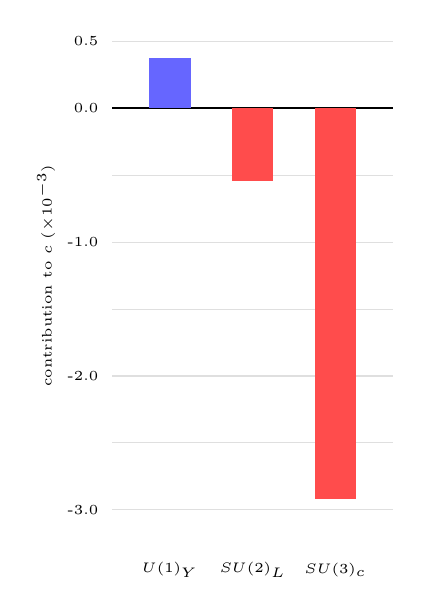
\begin{tikzpicture}[x=1.05cm,y=1.7cm]
  \foreach \y in {0.5,0.0,-0.5,-1.0,-1.5,-2.0,-2.5,-3.0}
    \draw[gray!25] (-0.2,\y) -- (3.2,\y);
  \foreach \y in {0.5,0.0,-1.0,-2.0,-3.0}
    \node[left,font=\tiny] at (-0.25,\y) {\y};
  \draw[thick] (-0.2,0) -- (3.2,0);
  \fill[blue!60] (0.25,0) rectangle (0.75,0.3792);
  \fill[red!70] (1.25,-0.5437) rectangle (1.75,0);
  \fill[red!70] (2.25,-2.9170) rectangle (2.75,0);
  \node[font=\tiny] at (0.5,-3.45) {$U(1)_Y$};
  \node[font=\tiny] at (1.5,-3.45) {$SU(2)_L$};
  \node[font=\tiny] at (2.5,-3.45) {$SU(3)_c$};
  \node[font=\tiny,rotate=90] at (-1.0,-1.25) {contribution to $c$ ($\times 10^{-3}$)};
\end{tikzpicture}\\[4pt]
{\footnotesize (a) Level 1: $\kcancel=0.197$\\ $\net=-3.082\times10^{-3}$, $\gross=3.840\times10^{-3}$}
\end{minipage}
\hfill
\begin{minipage}{0.5\textwidth}
\centering
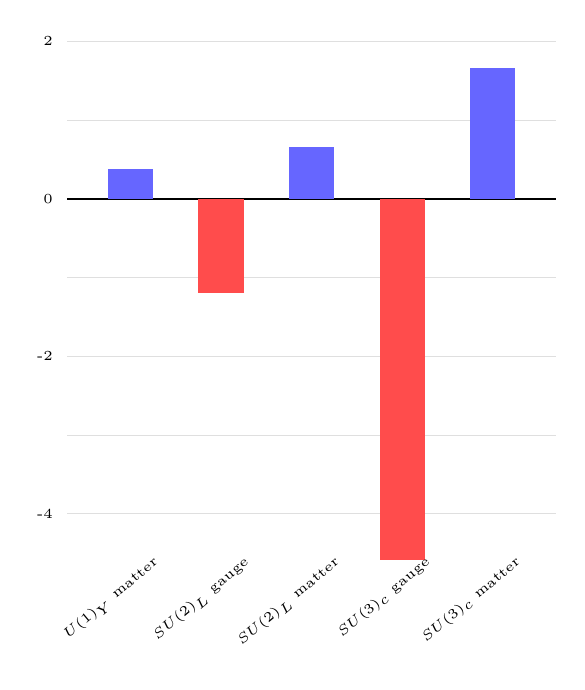
\begin{tikzpicture}[x=1.15cm,y=1.0cm]
  \foreach \y in {2,1,0,-1,-2,-3,-4}
    \draw[gray!25] (-0.2,\y) -- (5.2,\y);
  \foreach \y in {2,0,-2,-4}
    \node[left,font=\tiny] at (-0.25,\y) {\y};
  \draw[thick] (-0.2,0) -- (5.2,0);
  \fill[blue!60] (0.25,0) rectangle (0.75,0.3792);
  \fill[red!70] (1.25,-1.196) rectangle (1.75,0);
  \fill[blue!60] (2.25,0) rectangle (2.75,0.6525);
  \fill[red!70] (3.25,-4.584) rectangle (3.75,0);
  \fill[blue!60] (4.25,0) rectangle (4.75,1.667);
  \node[font=\tiny,anchor=north east,rotate=40] at (0.75,-4.35) {$U(1)_Y$ matter};
  \node[font=\tiny,anchor=north east,rotate=40] at (1.75,-4.35) {$SU(2)_L$ gauge};
  \node[font=\tiny,anchor=north east,rotate=40] at (2.75,-4.35) {$SU(2)_L$ matter};
  \node[font=\tiny,anchor=north east,rotate=40] at (3.75,-4.35) {$SU(3)_c$ gauge};
  \node[font=\tiny,anchor=north east,rotate=40] at (4.75,-4.35) {$SU(3)_c$ matter};
\end{tikzpicture}\\[10pt]
{\footnotesize (b) Level 2: $\kcancel=0.637$ (same net)\\ $\net=-3.082\times10^{-3}$ (unchanged), $\gross=8.479\times10^{-3}$}
\end{minipage}
\caption{The trace-anomaly coefficient at two resolutions. (a) The three gauge factors:
$\kcancel=0.197$, and the entire index is carried by the single positive $U(1)_Y$ channel, since
$\kcancel=2\min(P,N)/\gross$ and $P=c_{U(1)}$. (b) The gauge-boson/matter refinement of
\eqref{eq:level2}: identical net, larger gross, $\kcancel=0.637$. Neither value is more correct
than the other; each describes a stated resolution. Blue denotes positive contributions, red
negative. Values as in Table~\ref{tab:levels}.}
\label{fig:levels}
\end{figure}

\begin{remark}[Why the refinement does not empty the diagnostic]
\label{rem:survives}
Three things survive Theorem~\ref{thm:monotonicity} and Table~\ref{tab:levels}
(Figure~\ref{fig:levels}). First, the
direction of the effect is fixed, not arbitrary: by Theorem~\ref{thm:monotonicity}(iii) refinement
can only raise $\kcancel$, so level-1 values are lower bounds on the cancellation visible at any
finer resolution of the same object, and the statement ``at least a fifth of the mobilized gauge
magnitude does not appear in the net, at the coarsest gauge-factor resolution'' is well posed and
true. Second, the blindness statement strengthens rather than weakens under refinement: the
amplitude is a function of $\net$, which Theorem~\ref{thm:monotonicity}(i) shows is invariant under
the entire refinement hierarchy, so the amplitude is blind not to one alternative decomposition but
to all of them simultaneously. Third, the pair $(\net, \kcancel)$ remains a legitimate descriptor
of a \emph{stated} resolution, in the way that a coarse-graining scale is a legitimate parameter
rather than an embarrassment. What must be abandoned is the reading of $\kcancel$ as a number
attaching to the Standard Model; what replaces it is $\kcancel$ as a resolution-depth coordinate:
the pair $(0.20, 0.64)$ for levels 1 and 2 is more informative than either number alone, because the
gap between them is the amount of sign structure that the gauge-factor labelling conceals ---
unlike the algebraic witnesses of Remark~\ref{rem:witness}, this gap is realized by a refinement of
the same physical expression at fixed order and scale, and is therefore the one genuinely physical
comparison available at this order.
\end{remark}

\section{Consistency of the two readings}
\label{sec:consistency}

The first version of this note contained a tension it did not acknowledge. Reading~1 was built on
the plasma/$\beta$ factorization; Reading~2 computed $\kcancel$ on the unfactorized gauge channels.
But the $\beta$ factor is exactly where the additional sign structure lives
(Section~\ref{sec:level2}), so the first reading endorses a resolution the second ignores. One
cannot celebrate the factorization and then treat the unfactorized channel as the natural unit
without argument.

The present version resolves this by placing both readings on the two-level structure of
Proposition~\ref{prop:factorization} from the outset. Level~1 supports the amplitude's aggregation
statement; level~2 supports the tilt's factor-selection statement and supplies the refinement of
Section~\ref{sec:level2}. Observation~\ref{obs:blindness} is then a single statement about one
object at a stated resolution, and Table~\ref{tab:levels} reports both resolutions rather than
silently choosing one. The unified reading is:

\begin{quote}
Both Turok--Boyle observables are projections of a two-level signed structure that neither of them
resolves. The amplitude projects onto the magnitude of the signed sum across level-1 channels; the
tilt projects onto one level-2 factor of one level-1 channel. The descriptors $\gross$ and
$\kcancel$ quantify what is lost in the first projection, relative to a stated resolution, and are
monotone in that resolution.
\end{quote}

\section{Epistemic tiers}
\label{sec:tiers}

\paragraph{Tier 1 --- exact algebra, given the stated inputs.} Equation \eqref{eq:cbeta} as an
expression, and the numerical values of Tables~\ref{tab:levels} and~\ref{tab:scale} computed from
it. The uniform algebraic factorization $c_a=-P_a\alpha_a^2 b_a$ with $P_a>0$
(Proposition~\ref{prop:factorization}) and the sign attribution of Corollary~\ref{cor:signs}. (The
thermal reading of $P_a$ is Tier~2 for $SU(3)$ and is not claimed at all for the other two
channels; see Caution~\ref{caut:algebraic}.) The descriptor identities \eqref{eq:descriptors},
\eqref{eq:kappa-pn}. The condition-number identity of Proposition~\ref{prop:condition-number}. The
monotonicity theorem (Theorem~\ref{thm:monotonicity}) and the invariance audit of
Table~\ref{tab:audit}. The algebraic marginal-blindness of Proposition~\ref{prop:marginal-blindness},
with the caveat of Remark~\ref{rem:trivial}. That the signed decomposition is not a Fisher simplex
(Remark~\ref{rem:not-fisher}).

\paragraph{Tier 2 --- results imported from Turok and Boyle under their own stated assumptions.}
That $\mathcal{P}_\mathcal{R} \propto (c_\beta/N_{\mathrm{eff}})^2$, a derivation internal to a
framework this note does not assess. And, in particular, the tilt relation \eqref{eq:tilt} and the
plasma/$\beta$ interpretation of the two factors, which Turok and Boyle explicitly present as
heuristic and dependent on assumptions they state they have not verified. Any diagnostic reading of
the tilt inherits that status.

\paragraph{Tier 3 --- structural interpretation offered here, not established.} The reading of the
amplitude and tilt as two blindnesses of one object (Observation~\ref{obs:blindness}); the reading
of $\kcancel$ as a resolution-depth coordinate (Remark~\ref{rem:survives}); the suggestion that the
level-1/level-2 gap is a meaningful quantity rather than an artefact of a convenient split. These
are organizational proposals, falsifiable only in the weak sense that a better-motivated canonical
decomposition, if one existed, would displace them.

\paragraph{Tier 4 --- not claimed, and explicitly disavowed.} Any physical equivalence between the
signed-decomposition framework and the Turok--Boyle construction. Any derivation, validation,
extension, or critique of their result --- including any position on the pathologies identified by
\citet{ClineHell2026}. Any Fisher-geometric treatment of the signed decomposition absent an
explicit signed-context extension of the resolver theorem. Any reading of $\kcancel$ as a property
of the Standard Model, of the gauge sector, or of any physical system rather than of a stated
decomposition at a stated scale and truncation. Any reading of $\kcancel$ as a newly discovered
mathematical invariant, rather than the reparameterization of Proposition~\ref{prop:condition-number}.
Any suggestion that the numerical closeness of $\kcancel$ to $1/5$ is meaningful.

\section{Limitations}
\label{sec:limitations}

\begin{description}
\item[\textbf{(L1)}] \textbf{The formalism selects no unique resolution.}
Definition~\ref{def:descriptors} does not
privilege any decomposition, and Theorem~\ref{thm:monotonicity}(vi) shows $\kcancel$ spans $[0,1)$
over decompositions of a fixed net; hence no decomposition-independent value of $\kcancel$ is
established here. This is a statement about the formalism, not about physics: the gauge-factor
split is unusually natural, since the gauge group is a direct product and each factor contributes a
separately gauge-invariant operator, and it remains entirely possible that a physical argument
privileges one resolution. We claim only that the present framework supplies no such argument, and
that Section~\ref{sec:level2} exhibits a competing split drawn from the source paper itself.
\item[\textbf{(L2)}] \textbf{The descriptors are truncation-bound.} At higher order the decomposition into
independent single-gauge-factor channels ceases to be closed and canonical
(\citealp{MachacekVaughn1983,Mihaila2012}), because mixed-coupling terms require either additional
interaction channels indexed by pairs of factors or a convention for assigning them to one factor.
Either route is itself a resolution choice, and by Theorem~\ref{thm:monotonicity} introducing
interaction channels of either sign can only leave $\kcancel$ unchanged or raise it.
\item[\textbf{(L3)}] \textbf{The descriptors are scale-bound.} Two orders of magnitude separate the Planck and
electroweak values (Table~\ref{tab:scale}).
\item[\textbf{(L4)}] \textbf{The channel set is model-bound.} Under the emergent-Higgs hypothesis of
\citet{TurokBoyle2023}, no scalar channels appear at this order; see Remark~\ref{rem:higgs-doublet}
for exactly what that costs relative to the textbook Standard Model beta functions. That is an
assumption of their proposal, not a fact about the Standard Model, and relaxing it adds channels
and changes $\gross$ and $\kcancel$.
\item[\textbf{(L5)}] \textbf{The marginal-blindness proposition is near-trivial.} See Remark~\ref{rem:trivial}. The
framework's contribution is vocabulary and bookkeeping, applied to a specific physical coefficient,
not a theorem.
\item[\textbf{(L6)}] \textbf{The complementarity analogy is weaker than in the companion construction.} See
Caution~\ref{caut:complementarity}: the pair is nested rather than complementary, and
magnitude/log-derivative pairs are generic.
\item[\textbf{(L7)}] \textbf{Non-identifiability here is a statement about this diagnostic, not
about physical consistency.} That the amplitude
and tilt cannot jointly recover the signed channel decomposition, gross magnitude, or sign of
$c_\beta$ does not indicate any inconsistency in the Turok--Boyle construction; it indicates that
those two particular observables, as defined, are many-to-one functions of the underlying sum.
Whether some other observable resolves more of the decomposition is a separate, open question this
note does not address.
\item[\textbf{(L8)}] \textbf{Algebraic witnesses are not alternative physical realizations.} The two-component
construction of Theorem~\ref{thm:monotonicity}(vi), the global sign flip of
Remark~\ref{rem:logical-independence}, and the coupling-space witnesses of
Remark~\ref{rem:functional-independence} are constructed to prove mathematical statements about the
descriptors and the observation map. None of them describes an alternative Standard Model state,
and none should be read as such. Section~\ref{sec:level2}'s gauge-boson/matter refinement is the
one physically motivated comparison in this note.
\item[\textbf{(L9)}] \textbf{The underlying mechanism is contested in the refereed literature.} \citet{ClineHell2026}
identify pathologies in the dimension-zero scalar field construction that the Turok--Boyle
trace-anomaly analysis depends on. This note takes no position on that critique and does not need
to: the diagnostic below concerns what two stated observables reveal about a decomposition,
independently of whether the mechanism producing that decomposition survives further scrutiny.
\item[\textbf{(L10)}] \textbf{This note assesses no physics.} It records a coordinate reading of an external result
whose own status is contested and, in the tilt sector, explicitly provisional by its authors' own
account.
\end{description}

\section{Conclusion}
\label{sec:conclusion}

The trace-anomaly coefficient of \citet{TurokBoyle2023} is a signed, two-level object, ultimately
sourced from \citet{ArnoldZhai1995} for its functional form and \citet{Buttazzo2013} for its
numerical couplings: three gauge-factor channels, each factorizing exactly into a positive
prefactor --- thermal in origin for $SU(3)$ on the authors' reading, algebraically defined for the
other two (Caution~\ref{caut:algebraic}) --- and a one-loop-type $\beta$-coefficient combination
that is itself a difference of antiscreening and screening parts, and that coincides with the
textbook one-loop Standard Model beta function only because no fundamental Higgs doublet
contributes (Remark~\ref{rem:higgs-doublet}). The amplitude reads the magnitude of the signed sum
over level-1 channels, being an even function of it, and so discards both the decomposition and the
overall sign. Under the heuristic assumptions of \citet{TurokBoyle2023}, the tilt reads the
combination $b_3\alpha_3$ from one level-2 factor of one level-1 channel, independent of that
channel's positive prefactor and of the subdominant channels. Neither resolves the decomposition,
and their blindnesses are of different kinds.

The descriptors that quantify what is unresolved are classical, not new: $\net$ and $\gross$ are
the Jordan-decomposition total signed and total variation masses of a discrete signed measure
\citep{Bogachev2007}, and $\kcancel$ is an exact, bounded reparameterization of the condition number
of a sum \citep{Higham1993} (Proposition~\ref{prop:condition-number}). They are honest bookkeeping
but not invariants. Only the net is fixed once scale and truncation are fixed; the gross magnitude
and the cancellation index additionally require a stated decomposition, are monotone non-decreasing
under refinement, and range over all of $[0,1)$. Concretely, the value $\kcancel \approx 0.20$ at
the gauge-factor resolution becomes $0.64$ under the gauge-boson/matter refinement that
\citet{TurokBoyle2023} itself displays, and $0.002$ at the electroweak scale. The first version of
this note reported $0.20$ as though it characterized the Standard Model gauge sector; it does not,
and that claim is withdrawn.

What remains is worth stating precisely, and is all that is claimed. A net-only observable is
invariant under the entire refinement hierarchy of a signed decomposition, and therefore blind to
arbitrarily deep sign structure, provided that structure is reached by algebraic witnesses rather
than physically motivated refinements; $\kcancel$ is a monotone coordinate on that hierarchy, in
exact correspondence with the classical summation condition number, rather than a property of the
system; and the gap between the two physically meaningful resolutions available here --- gauge
factors and gauge-boson/matter, $0.20$ to $0.64$ --- measures how much sign structure a chosen
labelling conceals. The contribution is the systematic application of this classical vocabulary,
and the resulting identifiability audit, to one specific cosmological coefficient whose combination
of decomposition-, scale-, and truncation-dependence had not previously been examined this way. It
is not new mathematics, it is not new physics, and it is not a result about the Standard Model or
about the validity of the Turok--Boyle construction, which remains contested
(\citealp{ClineHell2026}; Limitation~L9).

\paragraph{Acknowledgments.} AI assistance was used for algebra checking, computation, figure
generation, manuscript drafting, literature and provenance organization, and adversarial review of
earlier drafts, including this revision. The invariance audit of Section~\ref{sec:audit}, the
alternative decomposition of Section~\ref{sec:level2}, the tier reassignment discussed in
Section~\ref{sec:tiers}, the correction of Caution~\ref{caut:sign-correction}, the condition-number
identification of Proposition~\ref{prop:condition-number}, and the explicit sourcing to
\citet{ArnoldZhai1995} and \citet{Buttazzo2013} all arose through AI-assisted review and a
subsequent, independently conducted literature and reproducibility audit of the accompanying
repository. No AI system is an author. All conceptual choices, claims retained, and final
responsibility for the work belong to the author.

\appendix
\section{Reproducibility}
\label{sec:reproducibility}

All numbers in this note follow from \eqref{eq:cbeta} and the couplings of Table~\ref{tab:scale}.
A reference implementation accompanies this manuscript at
\href{https://github.com/innerlightr-wq/signed-context-decomposition-cosmology}{github.com/innerlightr-wq/signed-context-decomposition-cosmology}. The canonical
module is the single top-level file \texttt{signedctx.py}; an earlier layout also carried a second,
superseded copy under \texttt{src/}, which the test harness imported by mistake under \texttt{pytest}
while the canonical module ran interactively --- this has been corrected, the duplicate removed,
and a regression test now guards against it recurring (see the repository's
\texttt{docs/CODE\_ARCHITECTURE.md}). No mathematics, physics input, or published number changed as
a result of that correction.

\begingroup\small
\begin{verbatim}
git clone \
    https://github.com/innerlightr-wq/signed-context-decomposition-cosmology.git
cd signed-context-decomposition-cosmology
pip install -r requirements.txt   # numpy, pytest

python signedctx.py               # self-check against this note's tables
python signedctx.py --levels      # both resolutions side by side
pytest -q                         # 62 tests, canonical module only
\end{verbatim}
\endgroup

\paragraph{What is exact algebra versus what is numerical.} The identities
\eqref{eq:descriptors}--\eqref{eq:condition-number}, the monotonicity theorem
(Theorem~\ref{thm:monotonicity}), and the sign attribution of Corollary~\ref{cor:signs} are proved
in this note and additionally checked symbolically/numerically by the module's self-check. The
entries of Tables~\ref{tab:levels} and~\ref{tab:scale} are floating-point evaluations of exact
rational coefficients at the quoted couplings and are exact to the precision shown; the module
reports them to full double precision. Example output:
\begingroup\small
\begin{verbatim}
level 1: net=-3.081767e-03  gross=3.840143e-03  kappa=0.197482
level 2: net=-3.081767e-03  gross=8.478969e-03  kappa=0.636543
\end{verbatim}
\endgroup
The $SU(3)$ share of $|\net|$ is $94.7\%$, consistent with the $95\%$ quoted by
\citet{TurokBoyle2023}.

\paragraph{Theorem~\ref{thm:monotonicity}(vi), a second witness.} Remark~\ref{rem:threshold}
illustrates unbounded growth of $\kcancel$ by splitting the strong channel itself. An independent
witness, using the same three level-1 values $c_1,c_2,c_3$ of Table~\ref{tab:levels} with an
\emph{injected}, unrelated canceling pair $(+X,-X)$ adjoined to the family (a refinement of the
zero vector, not of any existing channel), gives the same qualitative growth:
\begingroup\small
\begin{verbatim}
X=1e-3: kappa([c1,c2,c3,+X,-X]) = 0.4723
X=1e-2: kappa([c1,c2,c3,+X,-X]) = 0.8707
X=1e-1: kappa([c1,c2,c3,+X,-X]) = 0.9849
\end{verbatim}
\endgroup
independent of how the pair is attributed to a channel, confirming Theorem~\ref{thm:monotonicity}(vi)
by a second, structurally different construction. As with every construction in that theorem
(Remark~\ref{rem:witness}), this is an algebraic witness, not a physical decomposition.

\paragraph{What is exploratory and not part of any claim in this note.} The repository's third
example script runs an illustrative ensemble diagnostic over four \emph{hypothetical} gauge-sector
completions, to show what an ensemble test of Limitation~(L1) would look like. It certifies
nothing --- a single physical system cannot populate such an ensemble --- and no number from it
appears in this manuscript.

\bibliographystyle{plainnat}
\bibliography{references}

\end{document}
